\chapter{Estado del arte} \label{ch:estado_del_arte}

En este apartado lo que pretende es mostrar como se encuentra el panorama en el cual vamos a llevar a cabo nuestro proyecto. Para ello, en primer lugar realizaremos un análisis del mercado, donde se presentarán las principales alternativas a nuestra idea de proyecto ya existentes, de forma que analicemos los requisitos de nuestro sistema comparándolo con los de aquellos que ya existen. En segundo lugar analizaremos punto por punto los recursos utilizados para poder llevar a cabo este proyecto.

\section{Análisis de mercado}

En el Capítulo~\ref{ch:introduccion} comentábamos que el acceso a los datos ya era algo posible para toda la población. Esto se debe a que son de dominio público y es el propio gobierno de España o las Comunidades Autónomas los que publican los datos en sus respectivas web. Dado que este proyecto está centrado en la visualización de datos, es muy importante poder realizar una comparación de los requisitos que queremos presentar en el mismo con las diversas funcionalidades de otras aplicaciones englobadas dentro del mismo género. Por desgracia, tras realizar una búsqueda de aplicaciones en la \textbf{Play Store} de Google a fecha de Noviembre de 2020, el resultado mostrado a sido bastante sorprendente. Según \textbf{Play Store}, no hay ningún tipo de aplicación similar a lo que se pretende desarrollar en este proyecto. Ejemplo de ello son las aplicaciones que nos sugiere:

\begin{itemize}
	\item \textbf{Radar COVID:} Aplicación de alertas en caso de haber estado cerca de alguien que tiene COVID-19
	\item \textbf{GVA Coronavirus:} Aplicación de la Generalitat Valenciana para solicitar citas en caso de mostrar síntomas.
	\item \textbf{PassCOVIS.gal} Aplicación de la Xunta de Galicia para recibir avisos, información de las restricciones, recomendaciones y novedades.
	\item \textbf{COVIS-19.eus} Aplicación del Gobierno del País Vasco para realizar un auto-diagnóstico y avisar a tu círculo de personas.
	\item \textbf{CONFINAPP} Aplicación que pretende ser un acompañamiento y la puerta de entrada a la información y servicios de la Generalitat de Cataluña.
\end{itemize}

Visto que en el ámbito de las aplicaciones móviles no encontramos nada similar, tendremos que hacer una comparación con la principal fuente actual de información de la que disponemos, el \textbf{Gobierno de España}.

En este punto, antes que hacer el análisis, debemos conocer cuales son los requisitos que queremos tener en nuestra aplicación. Tras un estudio de los datos, siguiendo un criterio propio, he recogido las funcionalidades principales con las que debería contar una aplicación como la que se va a desarrollar y que permitan al propio usuario tener acceso a la misma sin ningún conocimiento previo. Estas funcionalidades por consiguiente sí están presentes en \textbf{Covid-19 Reports} y son las siguientes:

\begin{enumerate}
	\item Seleccionar la Comunidad Autónoma sobre la que se quieren conocer los datos.
	\item Visualización del incremento de casos, casos acumulados, media de la última semana y últimas 24h.
	\item Visualización de los fallecimientos acumulados, media de la última semana y últimas 24 horas.
	\item Visualización de los datos de hospitalización, camas y camas UCI ocupadas, porcentaje del total de camas, altas e ingresos.
	\item Visualización de casos y muertes según la edad, solo al consultar datos de España.
	\item Visualización de los casos por cada 100mil habitantes, solo al consultar datos de España.
	\item Visualización de los casos por cada 100mil habitantes en la última semana, solo al consultar datos de España.
	\item Visualización de los fallecidos por cada 100mil habitantes, solo al consultar datos de España.
	\item Visualización de los fallecidos por cada 100mil habitantes en la última semana, solo al consultar datos de España.
	\item Visualización ordenada y clara.
	\item Toda la información es gratuita.
	\item No tiene ampliaciones de pago.
	\item No tiene anuncios.
	\item Plataforma móvil donde se ofrece
\end{enumerate}

\subsection{Representación de datos Covid-19 en España}

Como hemos dicho antes, llevaremos a cabo un análisis de como se representan los datos por parte del \textbf{Gobierno de España}. Para ello tendremos que acceder a la página web de \textbf{Gobierno de España}, donde podemos consultar los datos del conjunto del territorio español. Teniendo en cuenta que no se trata de una aplicación si no de una web, se ha creído conveniente que los puntos 11-14 no es necesario analizarlos.

A primera vista el acceso a la información desde el navegador aparenta ser sencillo. El usuario tiene que acceder a la web de La Moncloa \cite{la-moncloa}, desde ahí se accederá a una pequeña pestaña llamada \textit{Covid-19}, la cual mostrará una serie de opciones, como se puede ver en la Figura \ref{fig:inicio-moncloa} y cuya opción a seleccionar será \textit{Cifras de la situación}.

\begin{figure}[H]
	\centering
	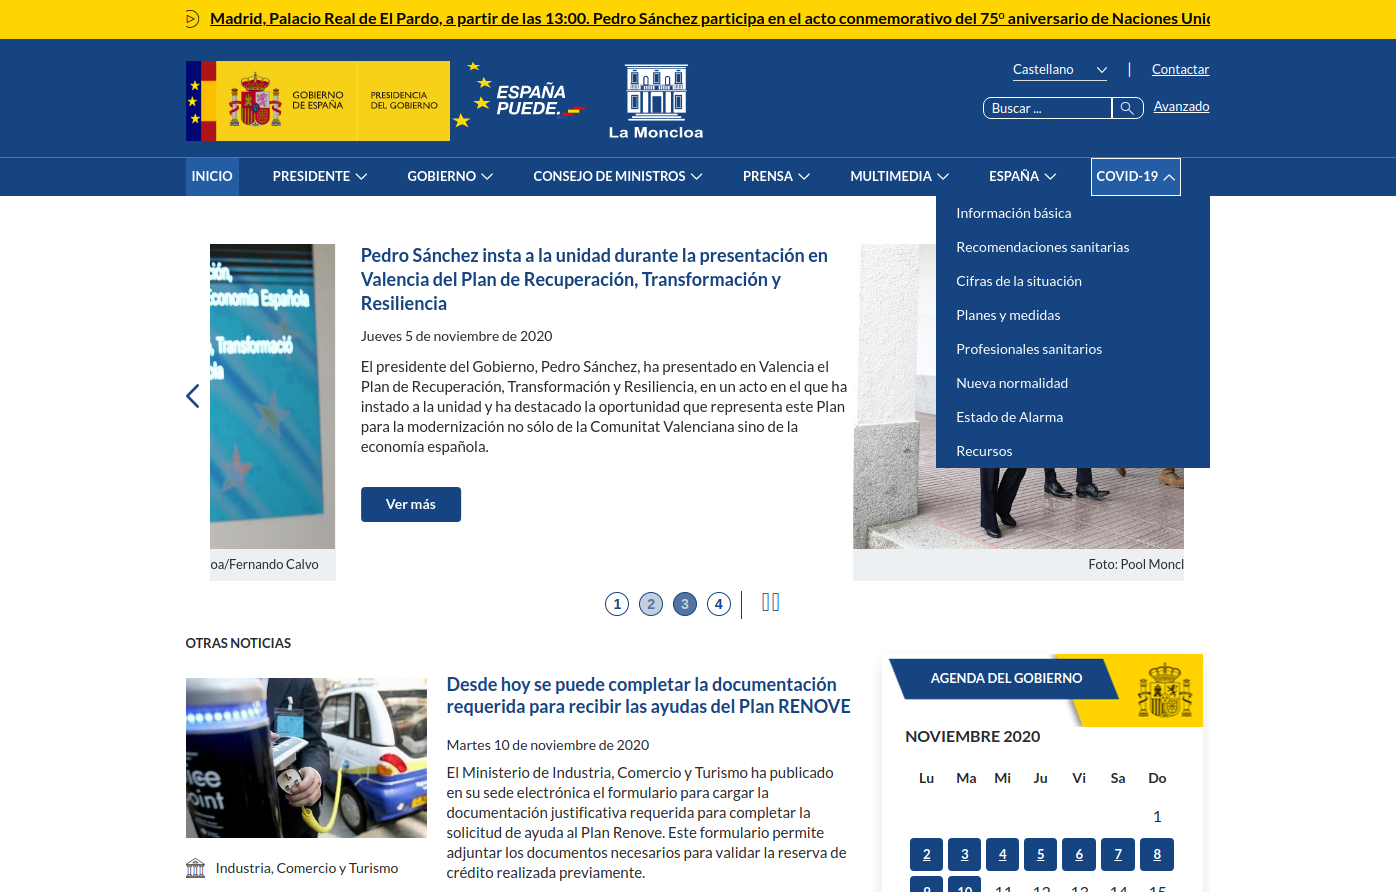
\includegraphics[width=1\textwidth]{img/inicio-moncloa}
	\caption{Página de inicio La Moncloa.}
	\label{fig:inicio-moncloa}
\end{figure}

\newpage
Una vez se ha redirigido al usuario, se le dará la opción de consultar los datos de España o los datos globales, junto con la opción de visualizar un video del proceso de recogida los datos en España, como se muestra en la Figura \ref{fig:opciones-moncloa}. Para este caso, la opción sobre la que nos centraremos es concretamente la que nos permite acceder a los datos a nivel de España, el usuario la seleccionará y será redirigido a una web del Ministerio de Sanidad \cite{gob-espana}, la cual vemos en la Figura \ref{fig:ministerio-salud}.

\begin{figure}[H]
	\centering
	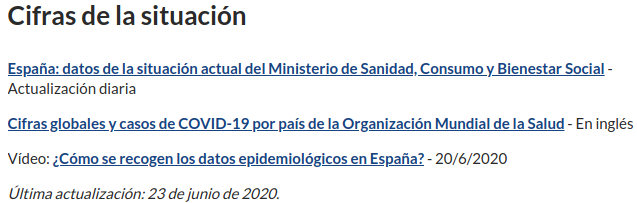
\includegraphics[width=1\textwidth]{img/opciones-moncloa}
	\caption{Opciones de consulta de La Moncloa.}
	\label{fig:opciones-moncloa}
\end{figure}

\begin{figure}[H]
	\centering
	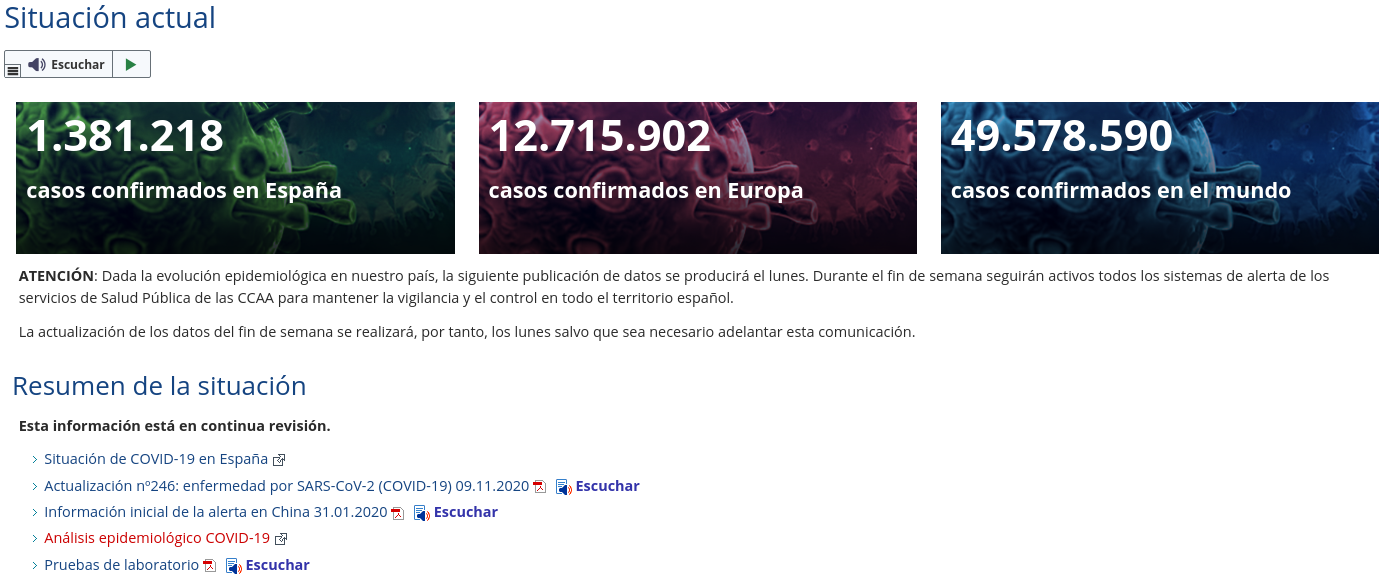
\includegraphics[width=1\textwidth]{img/ministerio-salud}
	\caption{Página de consulta del Covid-19 del Ministerio de Sanidad.}
	\label{fig:ministerio-salud}
\end{figure}

Dentro de la página del Ministerio de Sanidad lo primero que llama la atención y más resalta es el total de casos confirmados a nivel de España, de Europa y del Mundo. Además se indica al usuario que los datos, debido a la situación excepcional, se publicarán los lunes, de manera que la evolución de estos se verá semanalmente. Dentro de las opciones que se permiten seleccionar, el usuario tendrá seleccionar dos de ellas, en primer lugar \textit{Situación de COVID-19 en España}, la cual redirigirá al usuario a un mapa del territorio español interactivo donde lo único que se podrá consultar será la incidencia acumulada de las Comunidades Autónomas en los últimos 7 y 14 días como se muestra en la Figura \ref{fig:mapa-situacion}.

\begin{figure}[H]
	\centering
	\includegraphics[width=1\textwidth]{img/mapa-situación}
	\caption{Mapa con la incidencia acumulada por Comunidades Autónomas.}
	\label{fig:mapa-situacion}
\end{figure}

Otras de las opciones que el usuario puede seleccionar es la \textit{Actualización nº X}, que le permitirá visionar un pdf donde se encuentra toda la información unificada en tablas y posteriormente una serie de gráficas asociadas a las mismas. Dentro de toda la información que se nos proporciona, podemos ver la siguiente repartida en diversas tablas:

\begin{itemize}
	\item Casos de COVID-19 confirmados totales, diagnosticados el día previo y diagnosticados o con fecha de inicio de síntomas en los últimos 14 y 7 días.
	\item Casos de COVID-19 que han precisado hospitalización e ingreso en UCI. 
	\item Situación capacidad asistencial y actividad Covid-19 en hospitales.
	\item Total de Pruebas diagnósticas realizadas.
	\item Casos de COVID-19 que han fallecido (total y con fecha de fallecimiento en los últimos 7 días).
	\item Nº de casos COVID-19 importados de otro país.
	\item Detalles de los quince países con más casos confirmados de Europa
	\item Casos confirmados de COVID-19 fuera de Europa.
	\item Detalles de los quince países con más casos confirmados fuera de Europa
\end{itemize}

Si se quiere ver el modelo con el que se muestra esta información podemos acceder desde aquí \cite{actualizacion-gob}.

Como se ha podido de ver en el análisis, el acceso a los datos que nos proporciona el \textbf{Gobierno de España} es más o menos sencillo, pero para la gente que apenas usa esta web, mostrar un archivo pdf donde se representen enormes tablas con diversos datos que, aunque relacionados, cuando superan cierta cantidad pueden llegar a ser confusos, y gráficas separadas por varias páginas de estas tablas de datos, no es la mejor práctica posible.

\subsection{Comparativa}

Una vez hecho el análisis de la única opción conocida que puede llegar a aportar datos similares a los que queremos mostrar con nuestra aplicación, procederemos a hacer una comparativa con los diferentes requisitos que definimos con anterioridad.

Como hemos dicho antes, no compararemos los puntos 11-14 porque estos se han considerado que están asociados a un aplicación móvil y no a una página web como es el caso. En cuanto a los requisitos restantes, en referencia al 1, es cierto que podemos ver los datos de las diferentes Comunidades Autónomas, pero al tratarse de un simple documento pdf es imposible realizar una selección de las mismas.

En cuanto al resto de requisitos (2-9), todos ellos son visibles dentro del documento que nos proporciona la página web. En cuanto al requisito 10, queda claro, como se ha mencionado antes, que la visualización tanto de datos y gráficas no es ordenada y mucho menos clara, sobre todo cuando se acumulan varios tipos de información.

Es cierto que en la información proporcionada por el \textbf{Gobierno de España} es muy completa, como debe esperarse de la máxima autoridad del país, pero eso no hace que sea perfecta. La principal idea de la aplicación que se va a desarrollar es poder facilitar el acceso a estos datos al usuario, permitiendole acceder de manera sencilla e intuitiva a los mismos y seleccionar la información que desea utilizar. Es decir, lo que se pretende es una aplicación sencilla e interactiva, cosa que no se nos proporciona por parte del \textbf{Gobierno de España}.

\section{Recursos necesarios} \label{sec:recursos}

\subsection{Telegram}

\begin{figure}[H]
	\centering
	
\includegraphics[width=0.2\textwidth]{img/telegram-icon}
	\caption{Logotipo de Telegram.}
\end{figure}

\textbf{Covid-19 Reports} está concebido para ser un chatbot, por lo que la primera decisión que se ha tenido que tomar ha sido la plataforma donde se implementará. Hay muchas aplicaciones sobres las que se podría llevar a cabo el desarrollo de este chatbot, aunque para este punto se han considerado solo dos de ellas: WhatsApp \cite{whatsapp} y Telegram \cite{telegram}. En un artículo de la web Xataka Android \cite{articulo-xataka}, se lleva a cabo una explicación punto por punto de las diferencias entre ambas aplicaciones finalizando con una tabla que mostramos en la Figura \ref{fig:tabla-comparativa}

\begin{figure}[H]
	\centering
	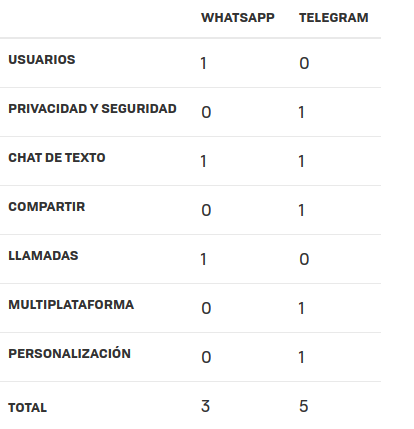
\includegraphics[width=0.6\textwidth]{img/tabla-comparativa}
	\caption{Tabla comparativa WhatsApp vs Telegram. Fuente: Xataka \cite{articulo-xataka}}
	\label{fig:tabla-comparativa}
\end{figure}

Existen varias razones por las que se ha optado por hacer uso de \textbf{Telegram}, entre ellas podemos destacar las siguientes:

\begin{enumerate}
	\item \textbf{Contenido disponible a través de Bots:} en el caso de \textbf{Telegram}, la lista de contenidos se ve multiplicada gracias a estos. Es cierto que \textbf{WhatsApp} también puede permitir la implementación de Bots, pero aún no es algo que se pueda realizar de manera generalizada, mientras que en \textbf{Telegram} cualquier usuario puede crear sus propios Bots.
	\item \textbf{Cuentas asociadas a un nº de teléfono:} \textbf{WhatsApp} tiene sus cuentas de usuario enlazadas a los números de teléfono de los usuarios, lo que implica que no se puede chatear con alguien sin tener su nº de teléfono. Sin embargo, \textbf{Telegram} facilita la comunicación entre usuarios asignándole nombres de usuarios a los mismos. Esto implica un importante punto a favor de \textbf{Telegram} en el ámbito de la privacidad, ya que en \textbf{WhatsApp} mientras formemos parte de un grupo todos los usuarios que se encuentre en este pueden ver nuestro nº de teléfono, \textbf{Telegram} mostrará en su lugar el nombre de usuario, impidiendo al resto conocer nuestro nº de teléfono.
	\item \textbf{Versión Web:} En este punto \textbf{Telegram} es el claro ganador. Aunque las dos aplicaciones cuentan con una versión Web, \textbf{WhatsApp} presenta un gran defecto que no se puede dejar pasar, y más a la hora de desarrollar una aplicación como esta: la estricta necesitad de tener el dispositivo móvil activo y conectado a Internet. En este aspecto, \textbf{Telegram} presenta una independencia total entre la versión de dispositivos y Web.
	\item \textbf{Descargas de contenido:} Sabiendo que queremos mostrar diferentes imágenes para favorecer el entendimiento de los datos a los usuarios, el evitar llenar la memoria de sus dispositivos es algo muy importante. \textbf{Telegram} almacena estos contenidos en la nube, por lo que no será necesario descargarlos para poder visionarlos, mientras que en \textbf{WhatsApp} por el contrario si queremos visualizar este contenido, tendríamos que permitir su almacenamiento en la memoria del dispositivo.
\end{enumerate}

\subsection{Python}

\begin{figure}[H]
	\centering
	
\includegraphics[width=0.2\textwidth]{img/python-icon}
	\caption{Logotipo de Python.}
\end{figure}

Como lenguaje de programación se ha optado por elegir \textbf{Python}. En primer lugar se debe a que es un lenguaje sobre el que he trabajado en varias ocasiones y es uno de los lenguajes más fáciles de manejar. Otra de las razones por las que he decidido trabajar en \textbf{Python} se debe a que a la hora de analizar datos y poder representarlos de manera gráfica, acciones que he podido probar en diversos lenguajes de programación y que \textbf{Python} permite realizar de manera más sencilla. Y no solo por ello, si no también por su popularidad. Según un artículo de Stackscale \cite{articulo-stackscale}, \textbf{Python} se ha convertido en el más utilizado, llegando a superar a \textbf{Java}, en los rankings de GitHub en 2019.

No solo por ello, se ha tenido en cuenta las características del proyecto y con que se va a trabajar. No solo es importante la interfaz del Bot, también lo es el contexto en el que trabajará, siendo en este caso el análisis de datos. Teniendo esto, aparece un nuevo lenguaje de uso común para el análisis de datos, \textbf{R}. Pero, ¿por que escogeremos a \textbf{Python} como el lenguaje principal de nuestro proyecto?

Según Paula Rochina en su artículo \cite{articulo-revista-digital} estas son las principales causas por las que debemos decantarnos por \textbf{Python}:

\begin{enumerate}
	\item \textbf{Python} es un lenguaje dinámico, lo que quiere implica que podremos cambiar el tipo de una variable o agregar nuevas propiedades o métodos a un objeto mientras el programa está en ejecución.
	\item La curva de aprendizaje de \textbf{Python} no es muy exigente, es un lenguaje sencillo de aprender tanto para nuevos programadores como para programadores que quieren incrementar las habilidades que tienen del mismo.
	\item Dado que el análisis de datos que se lleva a cabo en el proyecto no es independiente al mismo, si no que ha de estar integrado en nuestro Bot, \textbf{Python} es la mejor opción frente a \textbf{R}
\end{enumerate}

Para una mayor seguridad a la hora de elegir este lenguaje mencionaremos a artículo de Planeta CHATBOT, escrito por Marvin G. Soto \cite{articulo-planeta-chatbot} donde, como resumen, \textbf{Python} es la mejor alternativa para un chatbot al admitir todo tipo de funcionalidades y garantiza un acceso rápido y fácil a la información y los servicios de la aplicación como usuarios.

Una vez decidido sobre que lenguaje se va a desarrollar el proyecto explicaremos las diferentes librerías o paquetes que van a ser necesarios para poder desarrollar el Bot: python-telegram-bot, pandas y Matplotlib.

\subsubsection{python-telegram-bot}

\begin{figure}[H]
	\centering
	
\includegraphics[width=0.5\textwidth]{img/python-telegram-bot-icon}
	\caption{Logotipo de python-telegram-bot.}
\end{figure}

Se ha decidido escoger esta librería ya que proporciona al usuario una interfaz Python pura para el \textbf{Telegram Bot API}. Además de que es una librería que se actualiza con regularidad, ésta es compatible con las versiones más actuales de \textbf{Python}, siendo éstas las superiores a su versión 3.6. Además la biblioteca cuenta con algunas funciones para facilitar el desarrollo de Bots, haciéndolo mas fácil y sencillo.

Para mas información puede consultarse su repositorio en GitHub \cite{python-telegram-bot}

\subsubsection{pandas}

\begin{figure}[H]
	\centering
	
\includegraphics[width=0.2\textwidth]{img/pandas-icon}
	\caption{Logotipo de pandas.}
\end{figure}

la librería \textbf{pandas}, se considera una extensión de NumPy para poder manipular y analizar datos en \textbf{Python}. Se ha decidido utilizarla ya que previamente he trabajado con ella para aplicarla en ámbitos de Machine Learning, además en éste caso porque nos permite leer de manera fácil archivos de formato CSV (explicaremos más adelante porque hacemos uso de éstos archivos). También nos permite de una manera sencilla poder trabajar con tablas, acceder a sus índices, reordenarlas, modificarlas y combinarlas.

Para más información puede consultarse desde su web \cite{pandas}

\subsubsection{matplorlib}

\begin{figure}[H]
	\centering
	
\includegraphics[width=0.4\textwidth]{img/matplotlib-icon}
	\caption{Logotipo de Matplotlib.}
\end{figure}

\textbf{Matplotlib} es una librería de \textbf{Python} dedicada a la generación de gráficos por medio de datos. Ésta combina a la perfección con \textbf{pandas}. Durante principios de 2020 he tenido la oportunidad de trabajar con diferentes bibliotecas gráficas para \textbf{Python}, como Sklearn. Al trabajar con ambas al mismo tiempo me llegué a sentir mas cómodo con \textbf{Matplotlib}, ya que me parecía más sencilla de utilizar. Por ello se ha optado por su uso para este proyecto.

Para más información puede consultarse desde su web \cite{matplotlib}

\subsection{Git y GitHub}

\begin{figure}[H]
	\centering
	
\includegraphics[width=0.4\textwidth]{img/git-icon}
	\caption{Logotipo de Git.}
\end{figure}

\textbf{Git} es un software de control de versiones. Está pensado para la eficiencia y la confiablilidad del mantenimiento entre versiones de aplicaciones cuando éstas tienen un gran número de archivos de código fuente. \textbf{Git} nace de la necesidad de llevar un control de los cambios de los archivos y sobre el trabajo que diferentes personas puedan realizar sobre archivos que se encuentran compartidos en un proyecto.

\begin{figure}[H]
	\centering
	
\includegraphics[width=0.2\textwidth]{img/github-icon}
	\caption{Logotipo de GitHub.}
\end{figure}

\textbf{GitHub} es una plataforma que nos permite alojar proyectos haciendo uso del \textbf{Git}. Se ha decidido utilizar esta plataforma para alojar nuestro código ya que se pretende que sea un proyecto de software libre haciendo uso de una licencia \textbf{AGPL} \cite{agplv3}.

\subsection{Heroku}

\begin{figure}[H]
	\centering
	
\includegraphics[width=0.3\textwidth]{img/heroku-icon}
	\caption{Logotipo de Heroku.}
\end{figure}

Partiendo del punto en el que al crear un Bot para \textbf{Telegram} se obtienen unos TOKENS que son necesarios y están asociados al Bot en la aplicación y al ser un TOKEN que otorga manejo total sobre nuestro Bot no debe ser mostrado en ningún momento. Desde \textbf{Heroku} podremos proteger este TOKEN, permitiendo guardarlo con una variable de configuración, donde solo el dueño de la aplicación puede tener acceso a ellos y no son visibles en el código. \textbf{Heroku} es un PaaS (Platform as a Service) que nos permitirá poder desplegar nuestro Bot en la nube de manera que siempre esté en funcionamiento y podamos hacer uso de él en todo momento.

Para más información puede consultarse desde su web \cite{heroku}

A lo largo de este capítulo se ha podido observar y analizar los puntos importantes del arte de nuestro proyecto, comparando con otras aplicaciones o webs que pueden asimilarse a lo que se quiere llevar a cabo, así como las principales herramientas que se van a utilizar para desarrollar el mismo.